\subsection{Gantt Diagram}
\label{sec:gantt-diagram}

A Gantt diagram is attached at the end of this section. Continuous arrows represent Finish-Start (FS) dependencies between tasks, while dashed arrows represent Finish-Finish (FF) dependencies. FS dependencies indicate that successor tasks cannot start until their predecessor tasks are completed. FF dependencies show that successor tasks cannot finish until their predecessor tasks are completed.

Referring to Diagram \ref{fig:gantt-diagram} , the project timeline spans \textbf{122 days} with a \textbf{one-week built-in buffer}. Considering the 513 total estimated hours, this equates to approximately \textbf{4 hours of work per day}. Consequently, the weekly workload is 28 hours, matching the weekly effort allocated in the Gantt diagram. Hence, the task effort estimations from Table \ref{table:summary-of-tasks-with-effort-dependencies-and-resources} are translated into the Gantt diagram using this pattern (e.g., the ER1 task, which costs 20 hours, represents 4 days of work in the diagram).

According to Section \ref{sec:methodology}, regular meetings with the Product Owner are arranged every two days. Considering each meeting takes around 30 minutes, and that the project timeline spans 122 days, a total of 30.5 hours is dedicated to the \textbf{PM1} task. Consequently, these iterative meetings occur on the full Gantt diagram timeline, and \textbf{should be represented iteratively} as well. However, since the diagram tool does not support this behavior, it is represented as a single concurrent task. 


Excluding PM1, several other tasks are represented as concurrent, which corresponds to their actual occurrence:

\begin{itemize}[leftmargin=0.75cm, noitemsep]  
    \item \textbf{PM2} remains undetermined due to undefined thesis director meetings, representing iterative appointments throughout the project lifetime.
    \item \textbf{PM3} starts after \textbf{PS2} (temporal planning) is completed and runs concurrently with full application development, as the product backlog requires constant updates whenever new features or tasks are added.
    \item \textbf{FPD2} runs over the project stage to ensure consistency with final deliverables.
    \item \textbf{Dev5}, which depends on \textbf{Dev1} (beginning once the repository is created), spans most of the project duration to satisfy objective SO5 from Section \ref{sec:objectives}, as clean code requires ongoing, extensive documentation.
\end{itemize}

Certain development tasks also demand additional time. These tasks have an initial effort estimation of \textbf{8 hours (2 days of the Gantt diagram)}. Since these tasks face a high probability of experiencing significant challenges, the \textbf{remaining effort time} is allocated as a \textbf{buffer}.  

Notable examples include\textbf{ER1}, \textbf{ER3}, \textbf{UA2}, and \textbf{UA6}. \textbf{ER1}. \textbf{ER1} is the first coding task; \textbf{ER3} requires extensive coordination with frontend and backend; \textbf{UA2} requires a prior database record of the employee hierarchy; \textbf{UA6} marks the author's first experience implementing email notifications. Finally, \textbf{Backend Development} tasks similarly incur additional time costs. 

%Gantt diagram from Images/GanttDiagram.png
\begin{figure}[H]
    \centering
    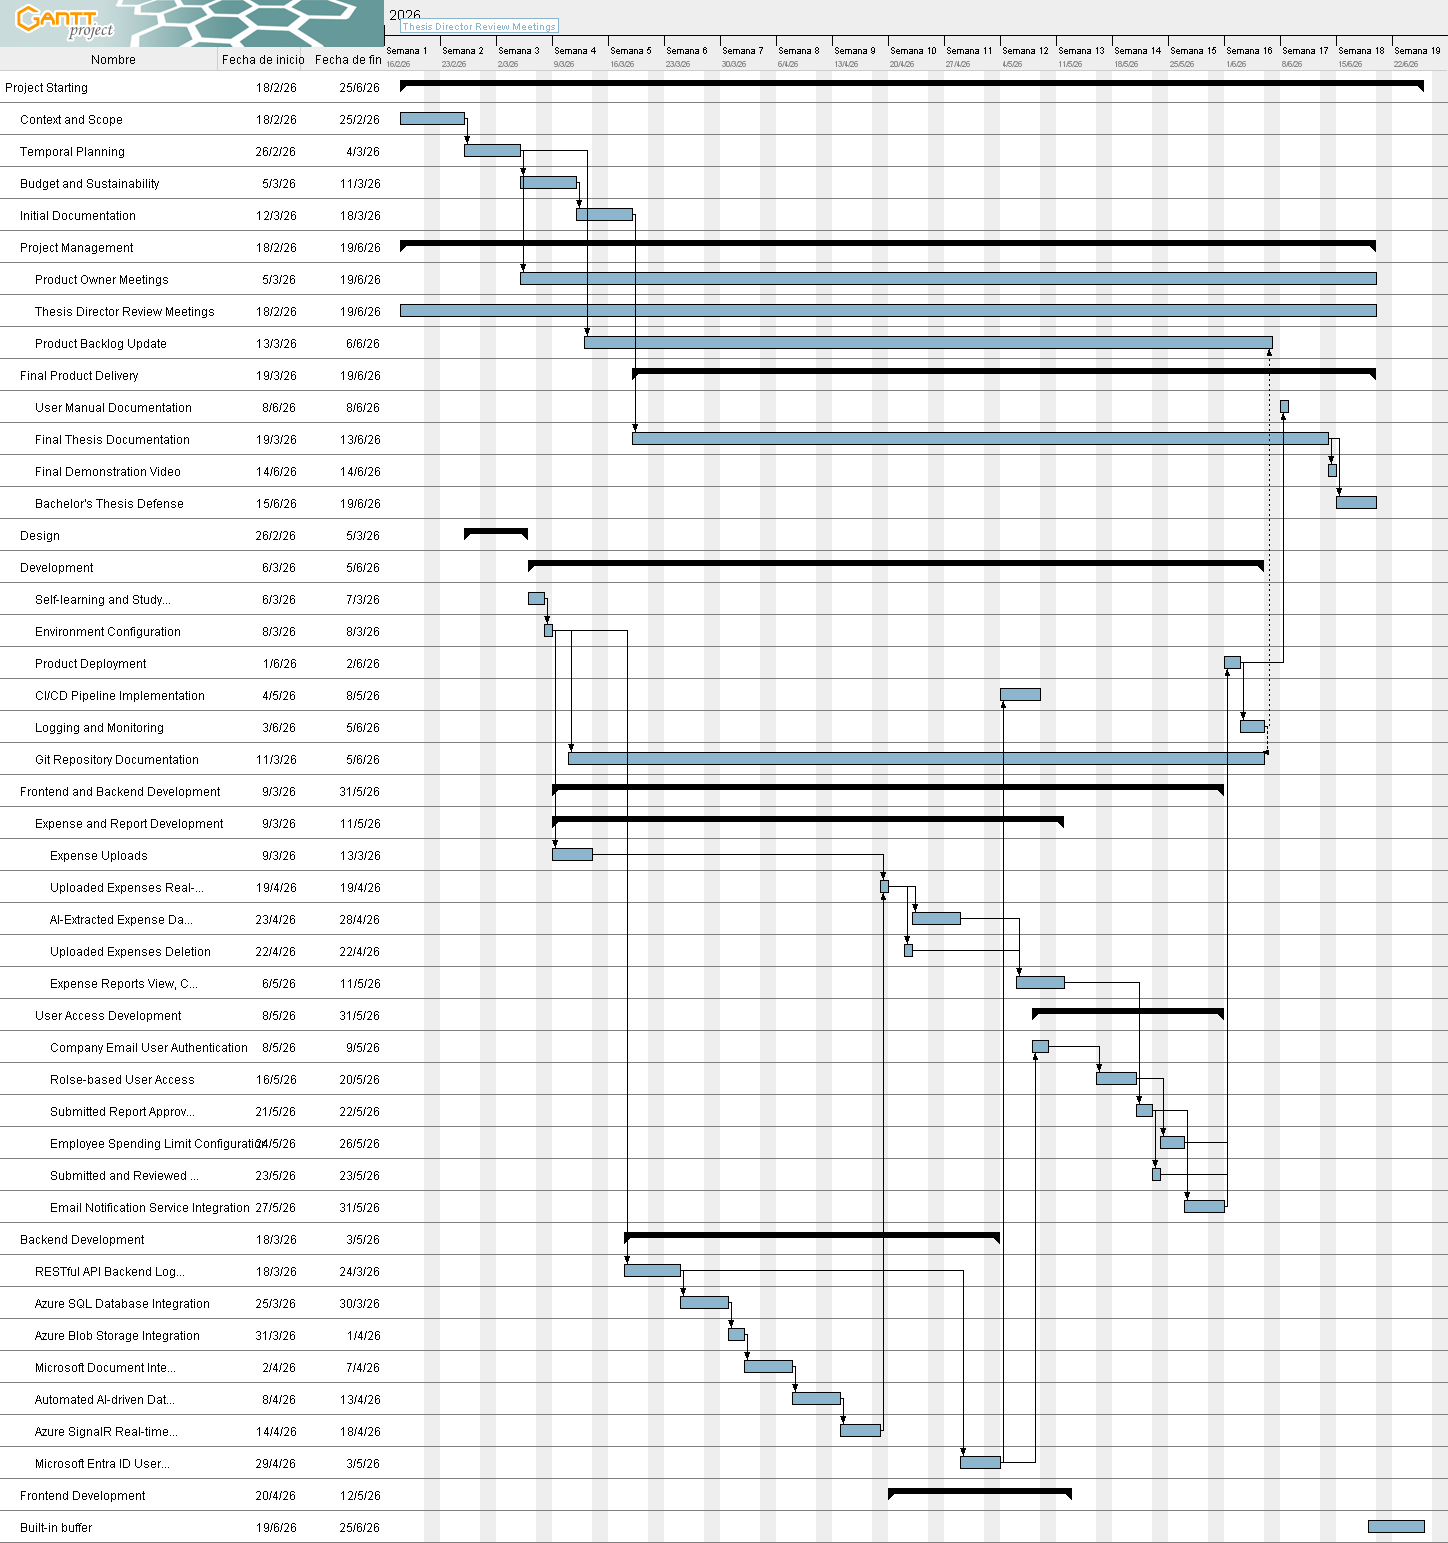
\includegraphics[width=\textwidth]{Images/GanttDiagram.png}
    \caption[Gantt Diagram.]
    {Gantt Diagram. [Own creation]} 
    \label{fig:gantt-diagram} 
\end{figure}    
